%%%%%%%% ICML 2018 EXAMPLE LATEX SUBMISSION FILE %%%%%%%%%%%%%%%%%

\documentclass{article}

% Recommended, but optional, packages for figures and better typesetting:
\usepackage{microtype}
\usepackage{graphicx}
\usepackage{subfigure}
\usepackage{booktabs} % for professional tables

\usepackage{amsfonts}
\usepackage{amsmath}

% hyperref makes hyperlinks in the resulting PDF.
% If your build breaks (sometimes temporarily if a hyperlink spans a page)
% please comment out the following usepackage line and replace
% \usepackage{icml2018} with \usepackage[nohyperref]{icml2018} above.
\usepackage{hyperref}

% Attempt to make hyperref and algorithmic work together better:
\newcommand{\theHalgorithm}{\arabic{algorithm}}

% Use the following line for the initial blind version submitted for review:
\usepackage[accepted]{icml2018}

% If accepted, instead use the following line for the camera-ready submission:
%\usepackage[accepted]{icml2018}

% The \icmltitle you define below is probably too long as a header.
% Therefore, a short form for the running title is supplied here:
\icmltitlerunning{A WaveNet Based Framework for Generating Singing Voice}

\begin{document}

\twocolumn[
\icmltitle{A WaveNet Based Framework for Generating Singing Voice \\
            (TAU Advanced Methods in ML course, 2018)}

% It is OKAY to include author information, even for blind
% submissions: the style file will automatically remove it for you
% unless you've provided the [accepted] option to the icml2018
% package.

% List of affiliations: The first argument should be a (short)
% identifier you will use later to specify author affiliations
% Academic affiliations should list Department, University, City, Region, Country
% Industry affiliations should list Company, City, Region, Country

% You can specify symbols, otherwise they are numbered in order.
% Ideally, you should not use this facility. Affiliations will be numbered
% in order of appearance and this is the preferred way.
\icmlsetsymbol{equal}{*}

\begin{icmlauthorlist}
\icmlauthor{Andrey Leshchenko}{equal}
\icmlauthor{Nir Raviv}{equal}
\icmlauthor{Roi Tabach}{equal}
\end{icmlauthorlist}

\icmlcorrespondingauthor{Nir Raviv}{nirraviv@mail.tau.ac.il}
\icmlcorrespondingauthor{Roi Tabach}{roi.tabach@gmail.com}
\icmlcorrespondingauthor{Andrey Leshchenko}{andrey.leshenko@gmail.com}


% You may provide any keywords that you
% find helpful for describing your paper; these are used to populate
% the "keywords" metadata in the PDF but will not be shown in the document
\icmlkeywords{Machine Learning, GAN, Generative Adversarial Networks, Singing Voice Generation}

\vskip 0.3in
]

% this must go after the closing bracket ] following \twocolumn[ ...

% This command actually creates the footnote in the first column
% listing the affiliations and the copyright notice.
% The command takes one argument, which is text to display at the start of the footnote.
% The \icmlEqualContribution command is standard text for equal contribution.
% Remove it (just {}) if you do not need this facility.

\printAffiliationsAndNotice{}  % leave blank if no need to mention equal contribution
% \printAffiliationsAndNotice{\icmlEqualContribution} % otherwise use the standard text.

\begin{abstract}
In 2016, Van Den Oord et al. presented WaveNet- a Deep neural network with the ability to generate raw audio waveforms.
Since than, there have been massive work in the area of Text to Speech and Speech to Text using WaveNet and its successors.
There has been some work regarding generating human singing voices, and we wanted to expand on that, as well as improve on their results.
We created a TTS based system that generates singing voice from a note track, with results better than the baseline, although not better than previous work.
\end{abstract}

\section{Introduction}
\label{introduction}
The goal of our project is to generate singing voices that sound as close to human as possible. 

Compared to text, the problem of creating singing voices is more complex, as the system has to generate matching pitch, timbre and melody.
Another problem is the lack of large datasets of professional recordings with timed lyrics.

Our overall approach to solving the problem is to use existing state-of-the-art systems for TTS, and training them on ``text'' which is made from a list of musical notes. We have a novel note detection method, built on top of the MELODIA pitch detection algorithm \cite{melodia}.
We then pass the musical notes stream, encoded as text, as the text that goes into the Tacotron 2 network.

The novelty in our work is twofold:
First by the way we extract the musical notes, and second by the novel usage of a working TTS system as a Notes-to-Singing system. 

\section{Related Work}
During the recent years many neural networks architecture based on fully-visible probabilistic autoregressive generative models are applied in many fields, such as natural images (PixelCNN) \cite{van2016conditional}, raw audio waveform (WaveNet) \cite{van2016wavenet} and video (Video Pixel Networks) \cite{kalchbrenner2016video}. These methods predict the distribution for each sample conditioned on all previous ones, while remaining efficiently trained.

Since WaveNet was published in 2016, there have been several major attempts at the problem of synthesizing speech with neural networks, including Deep Voice 1 \cite{arik2017deep}, 2 \cite{arik2017deep2}, and 3 \cite{ping2018deep}, Tacotron \cite{wang2017tacotron}, Char2Wav \cite{sotelo2017char2wav}, and others. Deep Voice 1 and 2 are built as TTS pipelines, separating grapheme-to-phoneme conversion, duration and frequency prediction, and waveform synthesis. Deep Voice 3, Tacotron and Char2Wav propose sequence-to-sequence models for neural TTS. Tacotron is a neural text-to-spectrogram conversion model, which uses Griffin-Lim \cite{griffin1984signal} for spectrogram-to-waveform synthesis. Char2Wav predicts the parameters of the WORLD vocoder \cite{morise2016world} and uses a SampleRNN \cite{mehri2016samplernn} conditioned upon WORLD parameters for waveform generation.
These works achieve state of the art performance, with human listeners rating as more natural sounding than the previous state of the art methods of concatenative methods.

Different singing generators are based on statistical parametric methods centered around Hidden Markov Models (HMM) which allow joint modeling of timbre and musical expression but perform less well than the previous methods by causing “buzzy” sound \cite{oura2012pitch}.
This work was extended to feed-forward DNNs \cite{nishimura2016singing}.

Merlijin {\em et al.} \cite{blaauw2017neural} presented a synthesizer which can generate synthetic singing voice given musical score and phonetic lyrics. They are using different models to learn phonetic timing, pitch and timbre combining autoregressive generative model with mixture density output, instead of softmax, which allows skewness or truncated distribution and multiple modes.

\section{Our Approach and Experiments}
Our overall approach to solving the problem is to use existing state-of-the-art systems for TTS, and to train them on "text" which is made from a list of musical notes.
Our pipeline looks as in Figure \ref{network-arch}.
We begin with several hours of relatively homogeneous recordings of singing voices.
We separate them to 5-second long clips.
We then split them to slices of 125 milliseconds and pass them through a pitch-detection program (the Essential audio analysis library \cite{essentia}).
We then use a novel approach in which we decide which musical note the pitch represents, and encode it as text.
The generated text stream, with each 5 second sample, is the (text, speech) pairs that are used in the training of the Tacotron 2 network.
\begin{figure}[ht]
	\vskip 0.2in
	\begin{center}
		{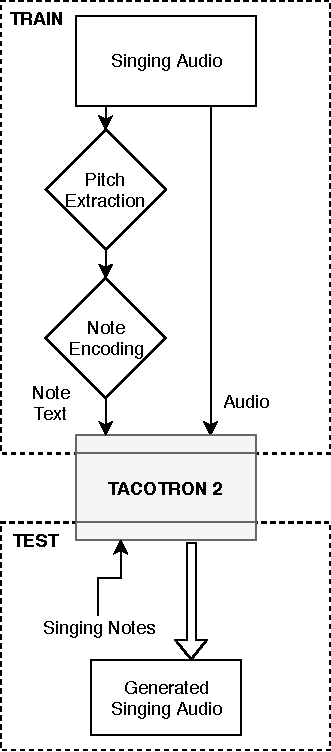
\includegraphics[width=0.7\columnwidth]{figures/network_arch.pdf}}
		\caption{The final Tacotron-2-based architecture of our singing system.
			At training we feed the network (text, audio) pairs where text
			is the pitch notes extracted from the audio.
			For testing we generate audio based on previously unseen singing notes.}
		\label{network-arch}
	\end{center}
	\vskip -0.2in
\end{figure}
\subsection*{Data Sets}
We have based our work on several data sets.
One of the closest works used a professional recording that was made by \cite{blaauw2017neural}.
They did not share their data with us, but Stanford university's DAMP dataset was in fact shared with us.

\subsubsection*{DAMP 300x30x2 \footnote{https://ccrma.stanford.edu/damp/}}
The DAMP dataset contains approximately $10^5$ audio recordings that were captured by Smule's Sing! Android karaoke application and hosted by the CCRMA.
The DAMP 300x30x2 is one of several subsets of those recordings.
It contains for each of 30 countries, the top 300 songs that users chose to sing inside the specific country.
For each song one recording by a male voice and one by a female voice.
Each recording usually contains only the singing voice itself, without the background music.
Naturally, this means that a large part of the recording is comprised of silence or background noises.
A large portion of the recordings has timed lyrics adjoined to them, some of them are timed by the sentence, some by the word, and some by the syllable.
Those timings come from the karaoke application, and the users are generally not precisely on time in their singing.
The dataset contains tags for some of the songs, with musical genres (e.g. k-pop, jazz, etc.).
There is also data for each of the users, including location, and number of followers.
When using the dataset we have noticed that our trained models generate various forms of silence and background noise.
This was somewhat solved using the following steps: working only on users with more than 10 followers, cutting the 5-second clips to coincide with the beginning of words, and adding fade-in and fade-out for clips that had sharp transitions.

A problem with DAMP we couldn't quite solve was the fact that it wasn't homogeneous enough, even after filtering by a specific genre and locale.
Many tracks had wrong M/F labels, others contained mostly silence and in some a person was just whispering the words instead of singing. It seems that this dataset could benefit greatly from human cleaning and supervision.
These problems, combined with the low quality of the recordings, convinced us to try working on different audio recordings.

\subsubsection*{Gregorian Chants \footnote{https://www.youtube.com/watch?v=xdroyjKs1Ls}}

In our search for high quality and homogeneous singing data,
we have turned to You Tube, where people often post hours-long music collections.
There we found a You Tube video containing six hours of Gregorian Chants \cite{gregorianVideo}.

Gregorian chant is a form of monophonic, unaccompanied sacred song, which developed mainly in western and central Europe during the 9th and 10th centuries. % cite Wikipedia ?
This dataset proved to be much more homogeneous, and the quality was higher than in DAMP.

\subsubsection*{LJSpeech}
As a part of the baseline, we have used the public LJ Speech dataset \cite{ito2017lj} that contains several hours of professional voice recordings of text.
The recording contains much less noise, and as expected generators trained on them gave much cleaner results.

\subsection*{Extracting the musical notes}	
Musical notes define the pitch of musical melodies, which is the quality that makes it possible to judge sounds as ``higher'' and ``lower'' \cite{plack2005pitch}.
In most cases the pitch will be the fundamental frequency of the signal, which is the frequency of repetition for a periodic waveform.
Calculating the fundamental frequency $f$ is complicated, because the harmonics of this frequency ($i \cdot f, \forall i \in \mathbb{N}$) can often be stronger than $f$.

We have attempted to extract the pitch from the STFT spectrograms of the audio tracks, but had many problems with strong harmonics being detected instead of the weaker fundamental frequency.
We then managed to get good results using the MELODIA algorithm \cite{melodia}, which is implemented as part of the Essential audio analysis library \cite{essentia}. 
\begin{figure}[ht]
	\vskip 0.2in
	\begin{center}
		{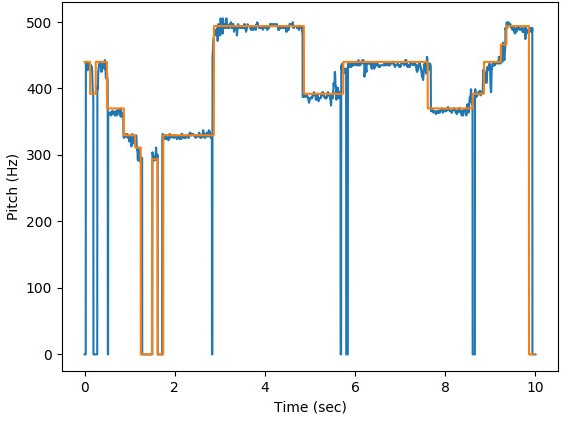
\includegraphics[width=0.7\columnwidth]{figures/pitch_detection.jpeg}}
		\caption{Pitch detection on a recording of a Gregorian Chant.}
		\label{pitch-detection}
	\end{center}
	\vskip -0.2in
\end{figure}
Figure \ref{pitch-detection} shows the results of pitch extraction on one of the Gregorian Chants tracks.
While it is possible to condition networks directly on the estimated pitch vectors,
we perform a further simplification of down-sampling the pitch values to 8 values per second,
and transforming the continuous frequencies into the discrete keys on a piano.
The piano is essentially a logarithmic scale, where the frequency is doubled every 12 keys.
Therefore, taking as a reference the A4 note as $f_0 = 440\text{Hz}$,
we can calculate the frequency of all other notes from their position $n$ relative to the base note:

$$
f_n = f_0 \cdot (\sqrt[12]{2})^n
$$

After pitch extraction we use the reverse of this formula to get the corresponding note:

$$
n = \lfloor\log_{\sqrt[12]{2}}\left(\frac{p}{f_0}\right) + 0.5\rfloor
$$

We then encode each note (from the 4 octaves where most singing occurs) as an uppercase or lowercase English letter.
For example, a pitch of 550 Hz will be detected as the note $C^{\#}_5$ (which has a frequency of 554.37 Hz)
and will be encoded as ``q''.

\subsection*{Tacotron 2 TTS}

The Tacotron 2 \cite{shen2017natural} is 
a neural network architecture for synthesizing speech directly from text.
We are abusing it, by entering the "text" we got from the musical notes.
It's composed of a recurrent sequence to sequence feature prediction network that maps character embeddings to Mel-scale spectrograms, followed by a modified WaveNet model acting as a vocoder to synthesize time-domain waveforms from those spectrograms.

We have trained both Tacotron 2 and all of our baselines on Titan Xp GPUs.
Each experiment was ran several hours (at least 12).

Audio outputs can be listened to in here: \href{http://bit.ly/tau_ml_svg}{Singing Voice Generation Samples on Google Drive}


\subsection*{Baseline}
We have implemented two baseline methods to compare our method with.
The first is a simple WaveNet GAN.
We have trained it for 12 - 48 hours on various subsets of DAMP and the Gregorian Chant datasets, as well as (for sanity check) LJ speech.
Also, We have trained Tacotron, based on the audio samples and their timings from the DAMP dataset.

\section*{Conclusion}
We presented a singing generator based on Tacotron 2 TTS system that trained over songs' musical notes as "text" and was conditioned over their pitch.

There are two natural ways to judge the quality of the outcome of a system that is designed to generate human sounding voices: comparison to previous state-of-the-art methods, and comparison to real human voices.

Our system generates audio that does not really sound human at all, and comparing it with human voices is hopeless.
Also, the existing state-of-the-art systems generate results that are much better than ours.
We have reached this conclusion even without the usage of mean opinion score tests, which is a common measuring way in the field of generating human speech.

We have however compared our system to the two baselines described above.
We find that the results are slightly better than those generated from the DAMP and Gregorian chants, but sound less human than LJSpeech.

An interesting observation is that the best results (e.g. "damp ha tikva.wav" in the samples folder) that we got in our Notes-to-Singing model were those that were trained on DAMP.
But there was a large group of notes tracks that the model did not "sing well", with problems such as singing that faded out to silence in the middle of the song.
This could be another testimony to the unbalanced or messy nature of the DAMP dataset, which means this method could achieve better results on a more professional dataset.

It is evident that there is an importance to having a clean, good quality recordings, with correct timings.
The better the dataset was in those metrics, the better the results sounded.

\section*{Future work}
The most obvious way to continue is trying to use a TTS system but adding another text channel, meaning using both correctly timed text and notes extracted in the way we did.
This requires having a singing voice dataset which is better than publicly available today.

Another option for the system is to try use tools from the image style transfer world, adapted to the audio domain.
There have been several works in this direction, but usually between several musical instruments and not between several tunes of a singing voice.

Another future venue that seems to suggest itself naturally from our representation for the musical notes is using tools from the domain of deep learning over text, to auto generate notes in the same style as those in our data sets, i.e. to compose music that would be in the same style as given audio samples.

\section*{Acknowledgments}
We gratefully acknowledge Prof. Amir Globerson and the course staff for their support and for letting us use the GPUs we ran on.
We also thank Smule Inc. for sharing with us the DAMP dataset, which is hosted at Stanford University's CCRMA. 
We thank Rayhane Mama and Igor Babuschkin, the developers of Git free versions of Tacotron 2 and WaveNet.

% In the unusual situation where you want a paper to appear in the
% references without citing it in the main text, use \nocite

\bibliography{final_project}
\bibliographystyle{icml2018}


\end{document}
